% !TEX program = xelatex
\documentclass[aspectratio=169]{ctexbeamer}
\usetheme{CambridgeUS}
\usepackage{amsmath, amssymb}
\usepackage[en-US]{datetime2}
% \usepackage{enumitem}
\usepackage{pgf, tikz}
\usetikzlibrary{positioning}
\tikzset{
    rednode/.style={
        circle,
        draw=red, % 边框颜色为红色
        fill=red!10, % 填充颜色为红色的 10%
        thick, % 边框加粗
        minimum size=0.75cm,
        inner sep=0,
        font=\bf\small
    },
    bluenode/.style={
        circle,
        draw=blue,
        fill=blue!10,
        thick, % 边框加粗
        minimum size=0.75cm,
        inner sep=0,
        font=\bf\small
    }
}
\usepackage{caption}
\usepackage{subcaption}
\captionsetup{labelfont=bf, labelsep=quad, font=footnotesize}
\captionsetup[sub]{labelsep=space}
\renewcommand{\figurename}{Figure}
\renewcommand{\tablename}{Table}
\usepackage{booktabs}
\usepackage[algoruled, linesnumbered]{algorithm2e}
\SetKwProg{Function}{Function}{}{end}
\SetFuncSty{textsc}
\SetArgSty{}
\algomargin=1em
\SetNlSty{textbf}{}{:}
\DontPrintSemicolon
\usepackage{listings}
\lstset{
    language = C++,
    breaklines = true,
    extendedchars = false,  % 解决代码跨页时,章节标题,页眉等汉字不显示的问题
    basicstyle = \ttfamily,
    keywordstyle = \bfseries,
    numbers = left,
    numberstyle = \small,
    frame = single,
    backgroundcolor = \color{lightgray!40!white},
    showstringspaces = false,
    tabsize = 4,
    commentstyle = \it\color{gray},
}
\title{Day 8: Binary Heaps \& Disjoint Set Forests}
\author{Tinghai Zhang}
\newcommand{\highlight}[1]{\textbf{\textit{#1}}}
\renewcommand{\leq}{\leqslant}
\renewcommand{\geq}{\geqslant}
\begin{document}
    \begin{frame}
        \maketitle
    \end{frame}

    \section{Binary heaps}

    \subsection{Priority queue ADT}

    \begin{frame}{Priority queue ADT}{Requirements}
        There are some items with \highlight{priority}, and we need an ADT which supports:

        \begin{itemize}
            \item The next item to access or remove is the \highlight{highest-priority} item.
            \item New items may be added \highlight{any time}.
        \end{itemize}

        One of common use cases: hospital emergency department.
    \end{frame}

    \begin{frame}{Priority queue ADT}{Two basic implementation}
        \begin{itemize}
            \item (Unsorted) array
            \begin{itemize}
                \item Enqueue: add new item at the end of the array, $\mathcal O(1)$.
                \item Dequeue: scan the array to find the highest-priority item, $\mathcal O(n)$.
            \end{itemize}
            \item Sorted array
            \begin{itemize}
                \item Enqueue: scan the array to find the right position for the new item, $\mathcal O(n)$.
                \item Dequeue: remove the last item, $\mathcal O(1)$.
            \end{itemize}
        \end{itemize}
    
        Entirely unsorted is too chaotic, but entirely sorted is unnecessary. A compromise is to use a \highlight{heap}.
    \end{frame}

    \subsection{Binary heaps}

    \begin{frame}{Binary heaps}{Definition}
        \highlight{Binary heaps} store items \highlight{partially sorted}. All the items are stored in a \highlight{binary tree}, which satisfies:
        \begin{itemize}
            \item The tree is \highlight{complete}, i.e. nodes in it are filled left-to-right on each level (row) of the tree.
            \begin{itemize}
                \item The tree is complete if and only if the array representation of the tree is filled from index 0 to $n-1$.
            \end{itemize}
            \item The tree is \highlight{heap-ordered}, i.e. the value of each node is \highlight{greater than or equal to} the values of its children. We call the property \highlight{max-heap} property. The \highlight{min-heap} property is defined similarly.
        \end{itemize}
    \end{frame}

    \begin{frame}{Binary heaps}{An example}
        \begin{figure}[!htbp]
            \centering
            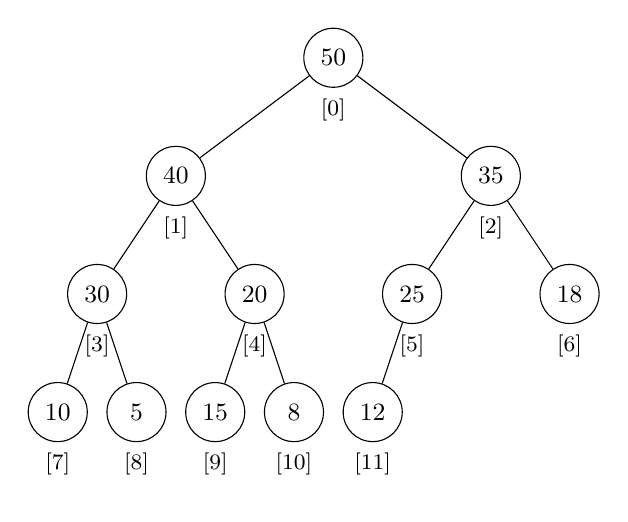
\begin{tikzpicture}[
                level distance=1.5cm, % 层与层之间的距离
                level 1/.style={sibling distance=4cm}, % 第一层节点之间的距离
                level 2/.style={sibling distance=2cm}, % 第二层节点之间的距离
                level 3/.style={sibling distance=1cm}, % 第三层节点之间的距离
                every node/.style={
                    circle, % 圆形节点
                    draw, % 绘制边框
                    minimum size=0.75cm, % 最小大小
                    inner sep=0, % 内边距为 0
                    font=\small % 字体大小
                }
            ]
            
            % 绘制大根堆的二叉树结构
            \node(0) {50} % 根节点
                child {
                    node(1) {40} % 左子节点
                    child {
                        node(3) {30} % 左子节点的左子节点
                        child { node(7) {10} }
                        child { node(8) {5} }
                    }
                    child {
                        node(4) {20} % 左子节点的右子节点
                        child { node(9) {15} }
                        child { node(10) {8} }
                    }
                }
                child {
                    node(2) {35} % 右子节点
                    child {
                        node(5) {25} % 右子节点的左子节点
                        child { node(11) {12} }
                        child [missing]
                    }
                    child { node(6) {18} }
                };
    
                \foreach \i in {0, ..., 11} {
                    \node [font=\footnotesize, below = -0.1cm of \i, draw=none] {[\i]};
                }
            \end{tikzpicture}
        \end{figure}
    \end{frame}

    \subsection{Implementation}

    \begin{frame}{Implementation}{Find parent and child nodes}
        \begin{algorithm}[H]
            \caption{Find parent and child nodes}
            \label{algo:Find parent and child nodes}
            \SetKwFunction{Parent}{Parent}
            \Function{\Parent{$i$}}{
                \Return{$\lfloor (i-1)/2\rfloor$}
            }
    
            \BlankLine
    
            \SetKwFunction{LeftChild}{Left-Child}
            \Function{\LeftChild{$i$}}{
                \Return{$2i+1$}
            }
    
            \BlankLine
    
            \SetKwFunction{RightChild}{Right-Child}
            \Function{\RightChild{$i$}}{
                \Return{$2i+2$}
            }
        \end{algorithm}
    \end{frame}

    \begin{frame}{Implementation}{Insert a new item}
        When inserting a new item into a max-heap, we add it to the end of the array and then \highlight{float} it up to keep the max-heap property. When floating up, we swap the new item with its parent until the max-heap property is satisfied.
    \end{frame}

    \begin{frame}{Implementation}{Insert a new item: Example}
        \begin{figure}[!htbp]
            \centering
            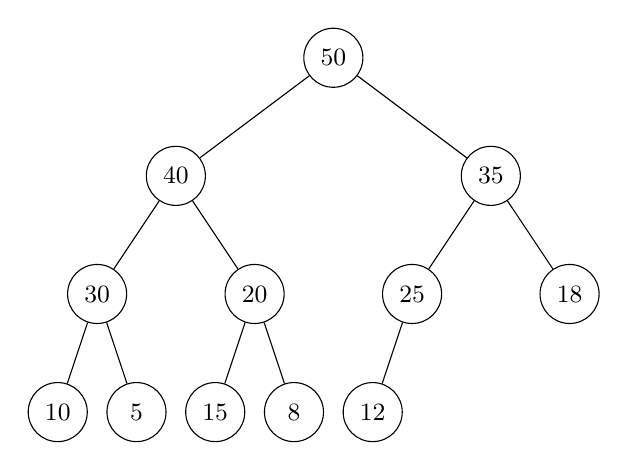
\begin{tikzpicture}[
                level distance=1.5cm,
                level 1/.style={sibling distance=4cm},
                level 2/.style={sibling distance=2cm},
                level 3/.style={sibling distance=1cm},
                every node/.style={
                    circle,
                    draw,
                    minimum size=0.75cm,
                    inner sep=0,
                    font=\small
                }
            ]
            % 初始大根堆
            \node {50}
                child {
                    node {40}
                    child {
                        node {30}
                        child { node {10} }
                        child { node {5} }
                    }
                    child {
                        node {20}
                        child { node {15} }
                        child { node {8} }
                    }
                }
                child {
                    node {35}
                    child {
                        node {25}
                        child { node {12} }
                        child[missing]
                    }
                    child { node {18} }
                };
            \end{tikzpicture}
        \end{figure}
    \end{frame}

    \begin{frame}{Implementation}{Insert a new item: Example}
        \begin{figure}
            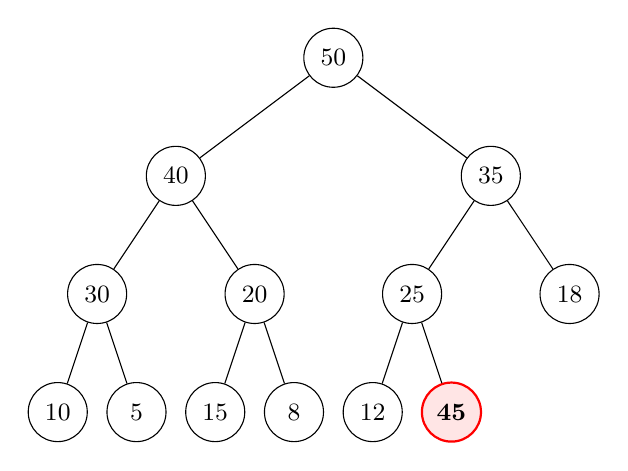
\begin{tikzpicture}[
                level distance=1.5cm,
                level 1/.style={sibling distance=4cm},
                level 2/.style={sibling distance=2cm},
                level 3/.style={sibling distance=1cm},
                every node/.style={
                    circle,
                    draw,
                    minimum size=0.75cm,
                    inner sep=0,
                    font=\small
                }
            ]
            % 初始大根堆
            \node {50}
                child {
                    node {40}
                    child {
                        node {30}
                        child { node {10} }
                        child { node {5} }
                    }
                    child {
                        node {20}
                        child { node {15} }
                        child { node {8} }
                    }
                }
                child {
                    node {35}
                    child {
                        node {25}
                        child { node {12} }
                        child { node[rednode] {45} }
                    }
                    child { node {18} }
                };
            \end{tikzpicture}
        \end{figure}
    \end{frame}

    \begin{frame}{Implementation}{Insert a new item: Example}
        \begin{figure}
            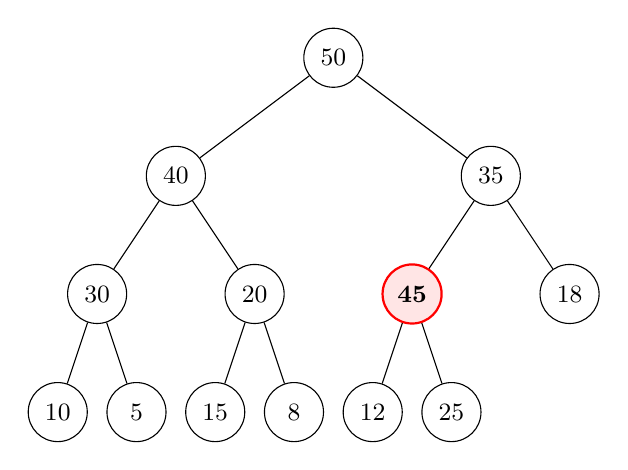
\begin{tikzpicture}[
                level distance=1.5cm,
                level 1/.style={sibling distance=4cm},
                level 2/.style={sibling distance=2cm},
                level 3/.style={sibling distance=1cm},
                every node/.style={
                    circle,
                    draw,
                    minimum size=0.75cm,
                    inner sep=0,
                    font=\small
                }
            ]
            % 初始大根堆
            \node {50}
                child {
                    node {40}
                    child {
                        node {30}
                        child { node {10} }
                        child { node {5} }
                    }
                    child {
                        node {20}
                        child { node {15} }
                        child { node {8} }
                    }
                }
                child {
                    node {35}
                    child {
                        node[rednode] {45}
                        child { node {12} }
                        child { node {25} }
                    }
                    child { node {18} }
                };
            \end{tikzpicture}
        \end{figure}
    \end{frame}

    \begin{frame}{Implementation}{Insert a new item: Example}
        \begin{figure}
            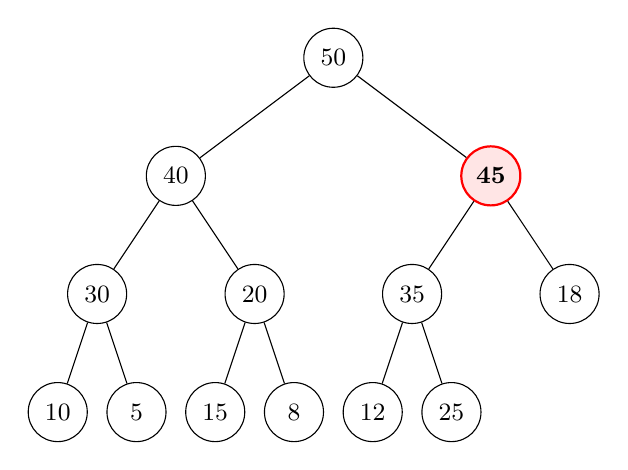
\begin{tikzpicture}[
                level distance=1.5cm,
                level 1/.style={sibling distance=4cm},
                level 2/.style={sibling distance=2cm},
                level 3/.style={sibling distance=1cm},
                every node/.style={
                    circle,
                    draw,
                    minimum size=0.75cm,
                    inner sep=0,
                    font=\small
                }
            ]
            % 初始大根堆
            \node {50}
                child {
                    node {40}
                    child {
                        node {30}
                        child { node {10} }
                        child { node {5} }
                    }
                    child {
                        node {20}
                        child { node {15} }
                        child { node {8} }
                    }
                }
                child {
                    node[rednode] {45}
                    child {
                        node {35}
                        child { node {12} }
                        child { node {25} }
                    }
                    child { node {18} }
                };
            \end{tikzpicture}
        \end{figure}
    \end{frame}

    \begin{frame}{Implementation}{Insert a new item: Algorithm}
        \begin{algorithm}[H]
            \caption{Add a new item to a max-heap}
            \label{algo:Add a new item to a max-heap}
            \SetKwFunction{Insert}{Insert}
            \SetKwFunction{FloatUp}{Float-Up}
            \Function{\Insert{$A,x$}}{
                \SetKwFunction{Pushback}{Push-back}
                $A.\Pushback(x)$\;
                \FloatUp{$A.\textit{size}-1$}\;
            }
            \BlankLine
            \Function{\FloatUp{$i$}}{
                \While{$i > 0$ and $A[i] > A[\Parent{$i$}]$}{
                    Swap $A[i]$ and $A[\Parent{$i$}]$\;
                    $i \gets \Parent{$i$}$\;
                }
            }
        \end{algorithm}
    \end{frame}

    \begin{frame}{Implementation}{Delete the highest-priority item}
        When deleting the highest-priority item from a max-heap, we first swap the root with the last item in the array, then \highlight{sink} the new root down to keep the max-heap property. The \highlight{sink-down} operation is similar to the \highlight{float-up} operation, but we swap the current node with its larger child until the max-heap property is satisfied.
    \end{frame}

    \begin{frame}{Implementation}{Delete the highest-priority item: Example}
        \begin{figure}
            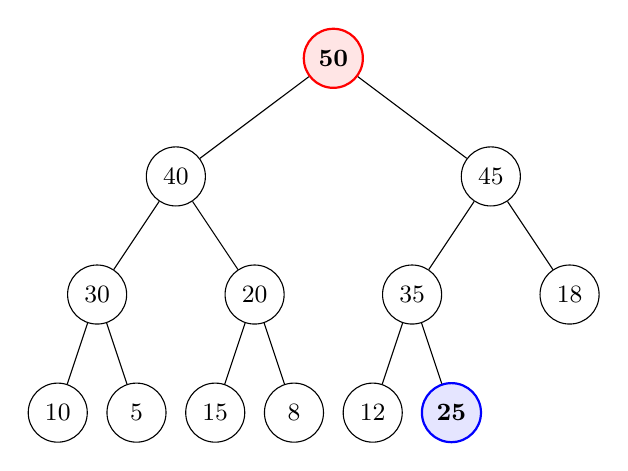
\begin{tikzpicture}[
                level distance=1.5cm,
                level 1/.style={sibling distance=4cm},
                level 2/.style={sibling distance=2cm},
                level 3/.style={sibling distance=1cm},
                every node/.style={
                    circle,
                    draw,
                    minimum size=0.75cm,
                    inner sep=0,
                    font=\small
                }
            ]
            % 初始大根堆
            \node[rednode] {50}
                child {
                    node {40}
                    child {
                        node {30}
                        child { node {10} }
                        child { node {5} }
                    }
                    child {
                        node {20}
                        child { node {15} }
                        child { node {8} }
                    }
                }
                child {
                    node {45}
                    child {
                        node {35}
                        child { node {12} }
                        child { node[bluenode] {25} }
                    }
                    child { node {18} }
                };
            \end{tikzpicture}
        \end{figure}
    \end{frame}

    \begin{frame}{Implementation}{Delete the highest-priority item: Example}
        \begin{figure}
            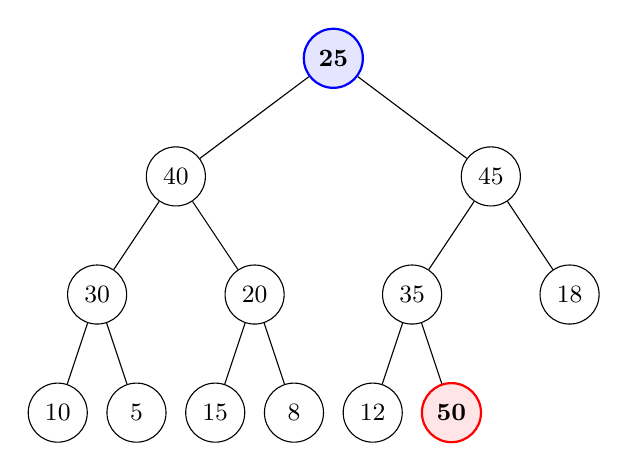
\begin{tikzpicture}[
                level distance=1.5cm,
                level 1/.style={sibling distance=4cm},
                level 2/.style={sibling distance=2cm},
                level 3/.style={sibling distance=1cm},
                every node/.style={
                    circle,
                    draw,
                    minimum size=0.75cm,
                    inner sep=0,
                    font=\small
                }
            ]
            % 初始大根堆
            \node[bluenode] {25}
                child {
                    node {40}
                    child {
                        node {30}
                        child { node {10} }
                        child { node {5} }
                    }
                    child {
                        node {20}
                        child { node {15} }
                        child { node {8} }
                    }
                }
                child {
                    node {45}
                    child {
                        node {35}
                        child { node {12} }
                        child { node[rednode] {50} }
                    }
                    child { node {18} }
                };
            \end{tikzpicture}
        \end{figure}
    \end{frame}

    \begin{frame}{Implementation}{Delete the highest-priority item: Example}
        \begin{figure}
            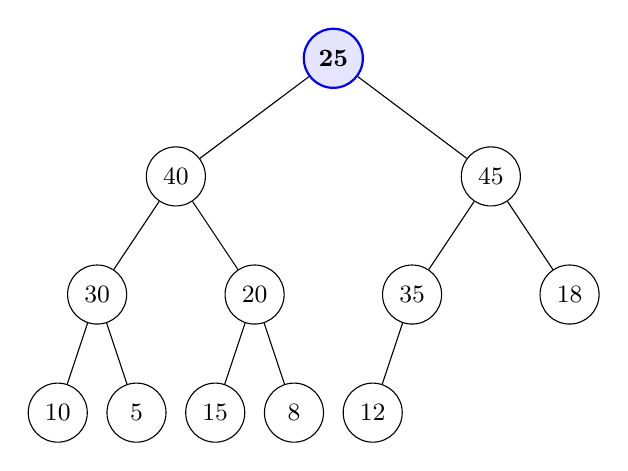
\begin{tikzpicture}[
                level distance=1.5cm,
                level 1/.style={sibling distance=4cm},
                level 2/.style={sibling distance=2cm},
                level 3/.style={sibling distance=1cm},
                every node/.style={
                    circle,
                    draw,
                    minimum size=0.75cm,
                    inner sep=0,
                    font=\small
                }
            ]
            % 初始大根堆
            \node[bluenode] {25}
                child {
                    node {40}
                    child {
                        node {30}
                        child { node {10} }
                        child { node {5} }
                    }
                    child {
                        node {20}
                        child { node {15} }
                        child { node {8} }
                    }
                }
                child {
                    node {45}
                    child {
                        node {35}
                        child { node {12} }
                        child[missing]
                    }
                    child { node {18} }
                };
            \end{tikzpicture}
        \end{figure}
    \end{frame}

    \begin{frame}{Implementation}{Delete the highest-priority item: Example}
        \begin{figure}
            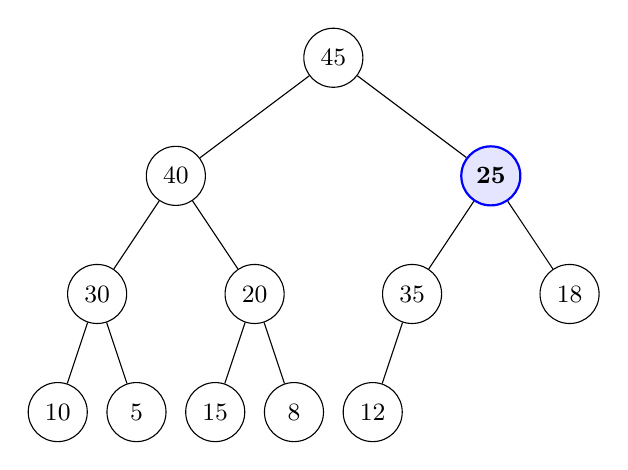
\begin{tikzpicture}[
                level distance=1.5cm,
                level 1/.style={sibling distance=4cm},
                level 2/.style={sibling distance=2cm},
                level 3/.style={sibling distance=1cm},
                every node/.style={
                    circle,
                    draw,
                    minimum size=0.75cm,
                    inner sep=0,
                    font=\small
                }
            ]
            \node {45}
                child {
                    node {40}
                    child {
                        node {30}
                        child { node {10} }
                        child { node {5} }
                    }
                    child {
                        node {20}
                        child { node {15} }
                        child { node {8} }
                    }
                }
                child {
                    node[bluenode] {25}
                    child {
                        node {35}
                        child { node {12} }
                        child [missing]
                    }
                    child { node {18} }
                };
            \end{tikzpicture}
        \end{figure}
    \end{frame}

    \begin{frame}{Implementation}{Delete the highest-priority item: Example}
        \begin{figure}
            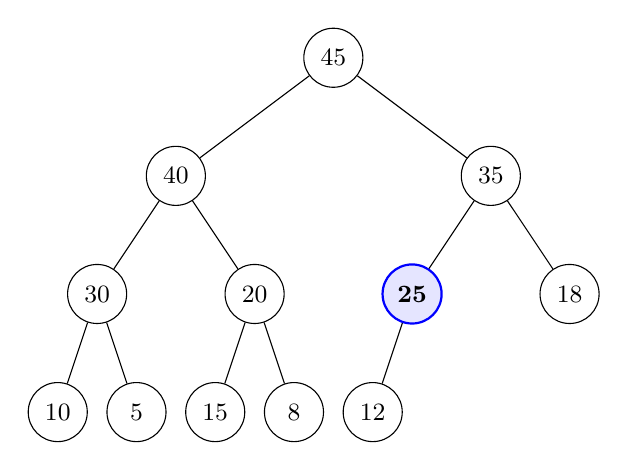
\begin{tikzpicture}[
                level distance=1.5cm,
                level 1/.style={sibling distance=4cm},
                level 2/.style={sibling distance=2cm},
                level 3/.style={sibling distance=1cm},
                every node/.style={
                    circle,
                    draw,
                    minimum size=0.75cm,
                    inner sep=0,
                    font=\small
                }
            ]
            \node {45}
                child {
                    node {40}
                    child {
                        node {30}
                        child { node {10} }
                        child { node {5} }
                    }
                    child {
                        node {20}
                        child { node {15} }
                        child { node {8} }
                    }
                }
                child {
                    node {35}
                    child {
                        node[bluenode] {25}
                        child { node {12} }
                        child [missing]
                    }
                    child { node {18} }
                };
            \end{tikzpicture}
        \end{figure}
    \end{frame}

    \begin{frame}{Implementation}{Delete the highest-priority item: Algorithm}
        \footnotesize
        \begin{algorithm}[H]
            \caption{Delete the highest-priority item from a max-heap}
            \label{algo:Delete the highest-priority item from a max-heap}
    
            \SetKwFunction{Delete}{Delete}
            \SetKwFunction{SinkDown}{Sink-Down}
            \Function{\Delete{$A$}}{
                \SetKwFunction{Popback}{Pop-back}
                Swap $A[0]$ and $A[A.\textit{size}-1]$\;
                $A.\Popback()$\;
                \SinkDown{$A,0$}\;
            }
            
            \BlankLine
    
            \Function{\SinkDown{$A,i$}}{
                \While{$\LeftChild{i} < A.\textit{size}$}{
                    $j \gets \LeftChild{i}$\;
                    \lIf{$j+1 < A.\textit{size}$ and $A[j+1] > A[j]$}{
                        $j \gets j+1$
                    }
                    \lIf{$A[i] \geq A[j]$}{\Return}
                    Swap $A[i]$ and $A[j]$\;
                    $i \gets j$\;
                }
            }
        \end{algorithm}
    \end{frame}
\end{document}